\chapter{Metoder}
\section{Litteratursøgning og metode}
\subsection{Litteraturstudie}
Undersøgelsens data og informationer er indhentet gennem litteraturstudier. Videnskabelig litteratur omhandlende videobaserede telesundhedsløsninger for hjemmepleje er søgt på følgende databaser: PubMed, Embase, CINAHL og Cochrane Library. Litteratursøgningsprocessen er udvidet til også at inkludere artikler identificeret ved kædesøgning i referencelister.\\
\begin{figure}[H]
\centering
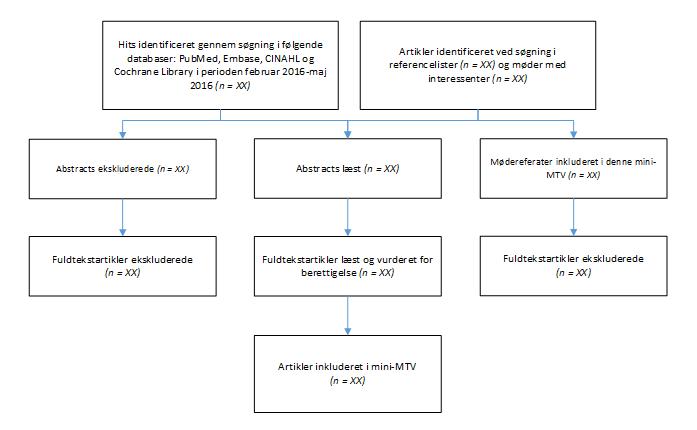
\includegraphics[width=1\textwidth]{Figurer/metode_flow.png}
\caption{\label{fig:metodeflow}Flowdiagram over  litteraturstudie. Flowdiagrammet angiver litteratursøgningsprocessen og identificerer antallet af ekskluderede og inkluderede artikler i MTV'en.}
\end{figure}

Emneord: Home Telemedicine, Telemedicine, Tele Care, Health Care, Tele Health Care.\\ \\
Ekskluderede artikler var telemedicinske problemstillinger vedrørende medicinsk behandling af patienter over distance. De inkluderede artikler omhandlede problemstillinger af telesundhedskarakter med fokus på virtuel hjemmepleje. 
Nedenstående tabel viser inkusionskriterne:
\begin{table}[H]
\caption{Inklusionskriterier}
\label{tab:inklusionstabel}
\centering
\begin{tabularx}{\textwidth}{lX}
\hline
Populationer/deltagere & Patienter, borgere og sundhedsprofessionelle uanset diagnose eller sundhedsforhold
Søgningen blev begrænset til studier i patienters/borgeres eget hjem
Der var ingen aldersbegrænsning af populationer/deltagere\\ \hline
Indsatser             & Informations- og kommunikationsteknologier (IKT) på sundhedsområdet        \\ \hline
Sammenligninger             & Fysisk hjemmeplejebesøg og virtuel hjemmeplejebesøg          \\ \hline
Udfald             & Sundhedsrelaterede udfald (livskvalitet, patient-/borgertilfredshed), procesudfald (sundhedsprofessionelles tilfredshed, kvaliteten af pleje)          \\ \hline
\end{tabularx}
\end{table}

På baggrund af inklusions- og eksklusionskriterierne er antallet af artikler inkluderet i denne mini-MTV n = XX. Samtlige artikler er udenlandske, men er vurderet repræsentative for denne mini-MTV, idet parametrene, som undersøges, er sammenlignelige med de udenlandske studier på området. En fuldstændig generalisering er ikke mulig, idet sundhedsforholdene varierer i de forskellige lande, så en fuldstændig sammenligning på tværs af landegrænser er ikke mulig. 

\subsection{Generel dataindsamling}
Data er endvidere indhentet gennem møder med forskellige interessenter – Appinux, Netplan Care og medarbejdere i Favrskov Kommune. Møderne har influeret på afgrænsningen af fokus, og på baggrund af disse møder er problemstillingen konkretiseret yderligere. Google i al almindelighed er ligeledes benyttet til indhentning af generel information om emnet telesundhed.

\subsection{Empirisk dataindsamling}
Med baggrund i de fokuserede spørgsmål har en stor del af fokus været på at belyse borgernes og sygeplejerskernes oplevelser og erfaringer med virtuel hjemmepleje. Det har derfor været nærliggende at supplere litteraturstudiet og den generelle dataindsamling med en kvalitativ interviewundersøgelse for netop at opnå en indgående og detaljeret viden herom.\\
I forbindelse med evalueringen af ’Pilotprojekt Videokommunikation’ blev der af Sundhedscenter Hadsten gennemført en lille kvalitativ evalueringsundersøgelse i form af strukturerede interviews med fire borgere og to sygeplejersker. Data fra denne interviewundersøgelse er indhentet og kritisk vurderet med henblik på anvendelse som empirisk datagrundlag i denne mini-MTV fremfor at igangsætte en ny empirisk videns indsamling.
\subsubsection{Diskussion af gyldigheden af den strukturerede interviewundersøgelse}
Gyldigheden af de otte på forhånd udformede spørgsmål i interviewundersøgelsen blev vurderet høj, idet indholdet af disse svarede overens med denne mini-MTV’s ønske om at opnå et fyldestgørende indtryk af borgernes og sygeplejerskernes oplevelser med videoopkaldene i virtuel hjemmepleje i Favrskov Kommune. Spørgsmålene lignede således meget de spørgsmål, som en ny empirisk interviewundersøgelse ville have indeholdt.\\ \\
Samlet set er den indhentede interviewundersøgelse fra ’Pilotprojekt Videokommunikation’ fra Sundhedscenter Hadsten vurderet gyldig, hvorfor det er valgt at medtage denne. En vigtig essens at pointere ved anvendelsen af interviewundersøgelsen er, at denne ikke efterlader mulighed for generalisering. Formålet med at anvende kvalitativ metode i dette konkrete tilfælde har været at undersøge borgernes og sygeplejerskernes oplevelser med brugen af videoopkald som alternativ til konventionel fysisk hjemmeplejebesøg i forhold til Appinux-løsningen i ’Pilotprojekt Videokommunikation’ fra Sundhedscenter Hadsten. Formålet har ikke været at lave et generaliserbart studie med resultater, som direkte kan overføres til andre lignende cases. Ved at sammenholde den empiriske dataindsamling med relevant videnskabelig litteratur samt viden indhentet ved møder med interessenter har det været muligt at opnå en dybere forståelse for borgernes og sygeplejerskernes perspektiv. 

\section{Referencesystem}
I denne mini-MTV anvendes Vancouver som referencesystem \cite{vancouver}.


\begin{table}[h]
\begin{tabular}{lcccccc}
& Lise & Sara & Melissa &Jeppe &Mohamed & Jakob\\
\midrule
Projektleder &  X & & & & &\\
\midrule
Borger/Organisation &X & X & X & & &\\
Ansvaret for Borger & &  & X& & &\\
Ansvaret for Organisation & & X&  & & &\\
\midrule
Teknologi/Økonomi & & & & X &  X & X\\
Ansvaret for Teknologi & & & & X & &\\
Ansvaret for Økonomi & & & & & &X\\

\end{tabular}
\end{table} 

  
	

